\documentclass[]{article}

\usepackage{hyperref}
\usepackage{caption}	% for \captionof 
\usepackage{tikz}		% for grids
\usepackage{pgfplots}   % for plot
\pgfplotsset{compat=1.18}

\title{HPCA-PC Exercise Sheet 2 --- Group 1}
\author{
	Mariia Isaeva\\
	\texttt{7910764}	\\
	\href{mailto:s6047802@stud.uni-frankfurt.de}{s6047802@stud.uni-frankfurt.de}
	\and
	Luiz Augusto da Silva Feitosa	\\
	\texttt{7890756}	\\
	\href{mailto:s1506025@stud.uni-frankfurt.de}{s1506025@stud.uni-frankfurt.de}
	\and
	Joshua Spingler\\
	\texttt{8243375}	\\
	\href{mailto:s7457265@stud.uni-frankfurt.de}{s7457265@stud.uni-frankfurt.de}
	\and
	Tim Wolf\\
	\texttt{7416419}	\\
	\href{mailto:s9677570@stud.uni-frankfurt.de}{s9677570@stud.uni-frankfurt.de}
}
\date{}

\begin{document}

\maketitle

\section*{Conway’s Game of Life}
\subsection*{Implementation}
	Our implementation follows an object-oriented approach with two main classes: \textit{World Class} (\texttt{World.h, World.cpp}), which manages the cellular automaton's state and evolution logic, and \textit{CLI Class} (\texttt{Cli.h, Cli.cpp}), which handles user interaction and command parsing.

\subsection*{File Organization}
	Our project follows a modular C++ structure with separation of headers, implementation files and a CMake build system.
	\begin{verbatim}
		game-of-life/
		|-- CMakeLists.txt              # CMake configuration
		|-- main.cpp                    # Application entry point
		|-- World.h                     # World class declaration
		|-- World.cpp                   # World class implementation
		|-- Cli.h                       # Cli class declaration
		|-- Cli.cpp                     # Cli class implementation
		\-- build/                      # Build directory (created)

	\end{verbatim}

\subsection*{Build Instructions}
	\begin{enumerate}
		\item \textbf{Configure project}:
		\begin{verbatim}
			mkdir build
			cd build
			cmake ..
		\end{verbatim}
		
		\item \textbf{Compile}:
		\begin{verbatim}
			make
		\end{verbatim}
		
		\item \textbf{Run}:
		\begin{verbatim}
			./main
		\end{verbatim}
		
		\item \textbf{Testing different optimization levels}:
		\begin{verbatim}
			# In CMakeLists.txt, change -O3 to:
			-O0  # No optimization (debugging)
			-O1  # Basic optimization
			-O2  # More optimization
			-O3  # Aggressive optimization
		\end{verbatim}
	\end{enumerate}

	\begin{center}
		\includegraphics[width=0.5\textwidth, height=0.9\textheight]{UML_Ex_02.png}
		\\[0.5em]
		\textbf{Figure 1: UML Class Diagram of Conway's Game of Life Implementation}
	\end{center}

	
\subsection*{Starting cell of multi-cell figures at the grid position (x,y)}
	All multi-cell patterns use the top-left corner as their anchor point $(x,y)$, marked with a red X in the diagrams below. When placing patterns using commands like \texttt{glider 5 5}, the pattern is positioned such that its top-left cell aligns with grid coordinates $(5,5)$. The toroidal grid behavior ensures that patterns wrap around the world boundaries. For example, placing a \textit{glider} at $(width-1, height-1)$ will cause parts of the pattern to appear at the opposite edges of the grid.

	\begin{center}
		% Glider
		\begin{minipage}{0.32\textwidth}
			\centering
			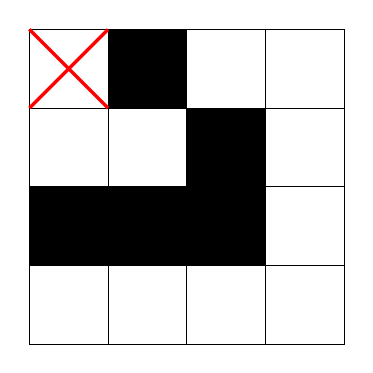
\begin{tikzpicture}
				\foreach \y in {0,...,3} {
					\foreach \x in {0,...,3} {
						\node[draw, minimum size=1cm] at (\x,-\y) {};
					}
				}
				\node[draw, minimum size=1cm, fill=black] at (1,0) {};
				\node[draw, minimum size=1cm, fill=black] at (2,-1) {};
				\node[draw, minimum size=1cm, fill=black] at (0,-2) {};
				\node[draw, minimum size=1cm, fill=black] at (1,-2) {};
				\node[draw, minimum size=1cm, fill=black] at (2,-2) {};
				
				\draw[red, very thick] (-0.5,0.5) -- (0.5,-0.5);
				\draw[red, very thick] (-0.5,-0.5) -- (0.5,0.5);
			\end{tikzpicture}
			\\[0.3cm]
			\textbf{Figure 2: Glider}
		\end{minipage}
		\hfill
		%Toad
		\begin{minipage}{0.32\textwidth}
			\centering
			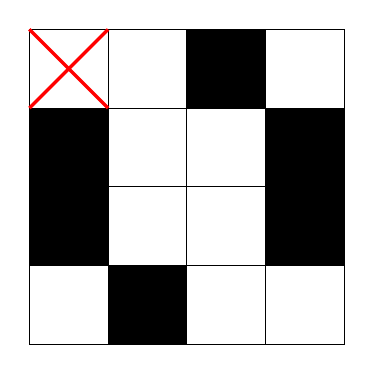
\begin{tikzpicture}
				\foreach \y in {0,...,3} {
					\foreach \x in {0,...,3} {
						\node[draw, minimum size=1cm] at (\x,-\y) {};
					}
				}
				\node[draw, minimum size=1cm, fill=black] at (2,0) {};
				\node[draw, minimum size=1cm, fill=black] at (0,-1) {};
				\node[draw, minimum size=1cm, fill=black] at (0,-2) {};
				\node[draw, minimum size=1cm, fill=black] at (1,-3) {};
				\node[draw, minimum size=1cm, fill=black] at (3,-1) {};
				\node[draw, minimum size=1cm, fill=black] at (3,-2) {};
				
				\draw[red, very thick] (-0.5,0.5) -- (0.5,-0.5);
				\draw[red, very thick] (-0.5,-0.5) -- (0.5,0.5);
			\end{tikzpicture}
			\\[0.3cm]
			\textbf{Figure 3: Toad}
		\end{minipage}
		\hfill
		% Beacon
		\begin{minipage}{0.32\textwidth}
			\centering
			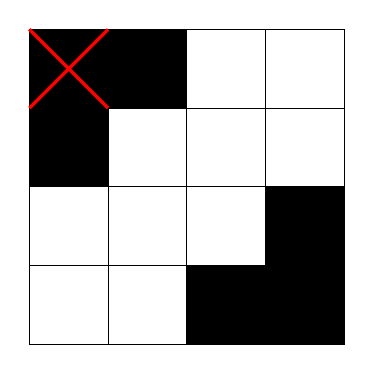
\begin{tikzpicture}
				\foreach \y in {0,...,3} {
					\foreach \x in {0,...,3} {
						\node[draw, minimum size=1cm] at (\x,-\y) {};
					}
				}
				\node[draw, minimum size=1cm, fill=black] at (0,0) {};
				\node[draw, minimum size=1cm, fill=black] at (1,0) {};
				\node[draw, minimum size=1cm, fill=black] at (0,-1) {};
				\node[draw, minimum size=1cm, fill=black] at (3,-2) {};
				\node[draw, minimum size=1cm, fill=black] at (2,-3) {};
				\node[draw, minimum size=1cm, fill=black] at (3,-3) {};
				
				\draw[red, very thick] (-0.5,0.5) -- (0.5,-0.5);
				\draw[red, very thick] (-0.5,-0.5) -- (0.5,0.5);
			\end{tikzpicture}
			\\[0.3cm]
			\textbf{Figure 4: Beacon}
		\end{minipage}
	\end{center}

\subsection*{Methuselah}
	We chose one of the smallest methuselahs, the \textbf{R-pentomino}, as our pattern. A small configuration (only 5 cells) that takes over 1,100 generations to stabilize. The anchor point (red X) marks the top-left position $(x,y)$ where the pattern is placed.
	
	\begin{itemize}
		\item \textbf{Pattern}: R-pentomino
		\item \textbf{Cells}: 5 live cells in 3×3 bounding box
		\item \textbf{Evolution}: Complex long-term behavior (1,103 generations)
		\item \textbf{Anchor}: Top-left corner at command coordinates
	\end{itemize}
	
	\begin{center}
		% Methuselah (R-Pentomino)
		\begin{minipage}{0.32\textwidth}
			\centering
			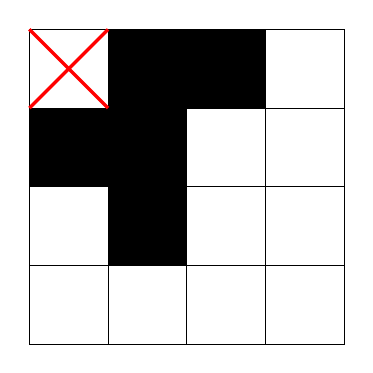
\begin{tikzpicture}
				\foreach \y in {0,...,3} {
					\foreach \x in {0,...,3} {
						\node[draw, minimum size=1cm] at (\x,-\y) {};
					}
				}
				\node[draw, minimum size=1cm, fill=black] at (1,0) {};
				\node[draw, minimum size=1cm, fill=black] at (2,0) {};
				\node[draw, minimum size=1cm, fill=black] at (0,-1) {};
				\node[draw, minimum size=1cm, fill=black] at (1,-1) {};
				\node[draw, minimum size=1cm, fill=black] at (1,-2) {};
				
				\draw[red, very thick] (-0.5,0.5) -- (0.5,-0.5);
				\draw[red, very thick] (-0.5,-0.5) -- (0.5,0.5);
			\end{tikzpicture}
			\\[0.3cm]
			\textbf{Figure 5: Methuselah}
		\end{minipage}
	\end{center}

\subsection*{CLI Features}
	\subsubsection*{Help System}
	Our CLI implementation includes a comprehensive help system accessible via the \texttt{help} or \texttt{h} commands. This system provides users with complete command reference and usage guidance.
	\\~\\
	\textbf{Help Command Output Structure:}
	\begin{verbatim}
		==================================================
		COMMAND REFERENCE
		==================================================
		
		WORLD MANAGEMENT:
		create <width> <height>    Create new world
		load <unix-path>           Load world from file
		save <unix-path>           Save world to file
		
		SIMULATION CONTROL:
		run <generations>          Run simulation
		print <0|1>                Toggle live display
		delay <milliseconds>       Delay between generations
		stability <0|1>            Auto-stop when stable
		
		CELL OPERATIONS:
		set <x> <y> <0|1>          Set cell state
		set <position> <0|1>       Set cell by 1D index
		get <x> <y>                Get cell state
		get <position>             Get cell by 1D index
		
		PATTERNS:
		glider <x> <y>             Add glider pattern
		toad <x> <y>               Add toad pattern
		beacon <x> <y>             Add beacon pattern
		methuselah <x> <y>         Add methuselah pattern
		random <count>             Add random patterns
		
		APPLICATION:
		help, h                    Command reference
		example, ex                Usage examples
		quit, q, exit, :q          Exit program
		==================================================
	\end{verbatim}
	
	\pagebreak
	
	\subsubsection*{Examples System}
	The \texttt{examples} or \texttt{ex} command provides practical usage scenarios to help users understand how to combine commands effectively.
	\\~\\
	\textbf{Examples Command Output Structure:}
	\begin{verbatim}
		==================================================
		USAGE EXAMPLES
		==================================================
		
		EXAMPLE 1: Basic simulation with visualization
		create 30 30       # Create 30x30 world
		glider 5 5         # Add a glider
		toad 15 10         # Add a toad oscillator
		print 1            # Enable live display
		delay 100          # 100ms between frames
		run 50             # Run 50 generations
		
		EXAMPLE 2: Fast simulation with stability check
		create 40 40
		random 8           # Add 8 random patterns
		print 0            # Disable display for speed
		stability 1        # Stop when world becomes stable
		run 1000           # Run up to 1000 generations
		
		EXAMPLE 3: Manual cell creation
		create 20 20
		set 5 5 1          # Create custom pattern
		set 6 6 1
		set 7 5 1
		set 7 6 1
		set 7 7 1
		print 1
		run 20
		
		EXAMPLE 4: Save and load workflow
		create 25 25
		glider 0 0
		beacon 10 10
		save my_pattern.txt
		# ... later ...
		load my_pattern.txt
		run 100
		==================================================
	\end{verbatim}
	
	\subsection*{Exercise 1.4: Optimization Level and Compilation Settings}
	
	The \texttt{print} to console and \texttt{is\_stable} checks were disabled.  
	The simulation ran with the file \texttt{p67\_snark\_loop.txt} for $n = 2000$ generations.
	
	\subsubsection*{Results}
	
	\begin{center}
		\begin{tabular}{|c|c|}
			\hline
			\textbf{Setting} & \textbf{Time [ms]} \\
			\hline
			\texttt{-O0} & 73 \\
			\texttt{-O1} & 73 \\
			\texttt{-O2} & 74 \\
			\texttt{-O3} & 75 \\
			\hline
			\texttt{Debug} & 446 \\
			\texttt{Release} & 75 \\
			\hline
		\end{tabular}
	\end{center}
	
	\subsubsection*{Discussion}
	
	Optimization levels \texttt{-O0} – \texttt{-O3} show negligible performance differences (73–75~ms).  
	The workload likely benefits little from compiler optimizations.
	
	In contrast, switching from \texttt{DEBUG} (446~ms) to \texttt{RELEASE} (75~ms) greatly improves speed,  
	as \texttt{DEBUG} mode includes extra checks and disables most optimizations.
	
	\subsubsection*{Conclusion}
	
	Optimization level has minimal effect, while compilation mode strongly influences performance.
	
	\subsection*{Exercise 1.5: Simulation Time per Grid Size}
	The \texttt{print} to console functionality and \texttt{is\_stable} check were disabled.  
	The simulation was compiled in \texttt{RELEASE} mode with optimization level \texttt{-O3}.  
	A blank world was used with a methuselah pattern placed at coordinates $(0, 0)$.  
	Each simulation ran for $n = 100$ generations.
	
	\subsubsection*{Results}
	
	\begin{center}
		\begin{tabular}{|c|c|}
			\hline
			\textbf{Grid Size (x, y)} & \textbf{Time [ms]} \\
			\hline
			(10, 10) & 0 \\
			(20, 20) & 0 \\
			(100, 100) & 4 \\
			(1000, 1000) & 355 \\
			(10000, 10000) & 35514 \\
			\hline
		\end{tabular}
	\end{center}
	
	\subsubsection*{Discussion}
	
	The simulation time increases rapidly with grid size.  
	Small grids complete almost instantly, while large grids require significantly more time.  
	This trend suggests an approximately quadratic scaling with the number of cells ($O(x \cdot y)$),  
	as each generation updates the entire grid.
	
	\subsubsection*{Plot}
	
	\begin{center}
		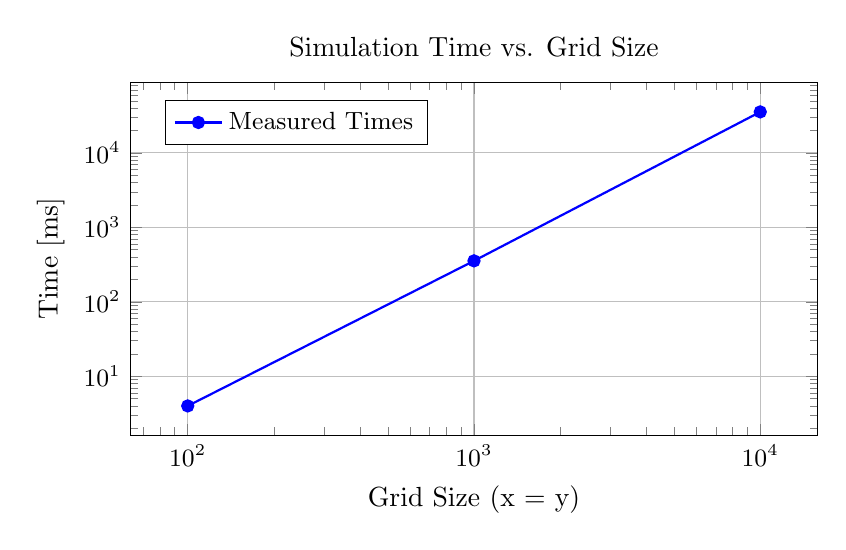
\begin{tikzpicture}
			\begin{axis}[
				width=0.85\textwidth,
				height=0.5\textwidth,
				xlabel={Grid Size (x = y)},
				ylabel={Time [ms]},
				title={Simulation Time vs. Grid Size},
				grid=major,
				ymode=log,
				xmode=log,
				log basis x=10,
				log basis y=10,
				tick label style={font=\small},
				legend style={font=\small, at={(0.05,0.95)}, anchor=north west}
				]
				\addplot[
				thick,
				mark=*,
				color=blue
				] coordinates {
					(10, 0)
					(20, 0)
					(100, 4)
					(1000, 355)
					(10000, 35514)
				};
				\addlegendentry{Measured Times}
			\end{axis}
		\end{tikzpicture}
	\end{center}
	
	\noindent
	\textit{Figure: Simulation time as a function of grid size (log–log scale).}
	

\end{document}
